
%(BEGIN_QUESTION)
% Copyright 2006, Tony R. Kuphaldt, released under the Creative Commons Attribution License (v 1.0)
% This means you may do almost anything with this work of mine, so long as you give me proper credit

A type ``K'' thermocouple is made of the dissimilar metals Chromel (chromium-nickel alloy) and Alumel (aluminum-nickel alloy).  Using a thermocouple table, determine the output voltages of a type ``K'' thermocouple at the following process temperatures:

$$\includegraphics[width=15.5cm]{i00368x01.eps}$$

\begin{itemize}
\item{} $T_{process}$ = 800$^{o}$ F; Voltmeter voltage = ??? 
\item{} $T_{process}$ = $-$163$^{o}$ F; Voltmeter voltage = ??? 
\item{} $T_{process}$ = 32$^{o}$ F; Voltmeter voltage = ??? 
\item{} $T_{process}$ = 2350$^{o}$ F; Voltmeter voltage = ??? 
\end{itemize}

\vskip 10pt

Also determine the standard color codes for type K thermocouple wire:

\begin{itemize}
\item{} Positive conductor:
\item{} Negative conductor:
\item{} Thermocouple-grade jacket:
\item{} Extension-grade jacket:
\end{itemize}

\vskip 20pt \vbox{\hrule \hbox{\strut \vrule{} {\bf Suggestions for Socratic discussion} \vrule} \hrule}

\begin{itemize}
\item{} Explain the rationale of using an ice-water bath for the reference junction.  Also, explain why both of the reference junction connections are immersed in ice-water baths instead of just one of them.
\end{itemize}

\underbar{file i00368}
%(END_QUESTION)





%(BEGIN_ANSWER)

\noindent
{\bf Partial answer:}

\medskip
%\item{} $T_{process}$ = 800$^{o}$ F; Voltmeter voltage = 17.526 mV 
\item{} $T_{process}$ = $-$163$^{o}$ F; Voltmeter voltage = $-$3.803 mV 
%\item{} $T_{process}$ = 32$^{o}$ F; Voltmeter voltage = 0 mV 
\item{} $T_{process}$ = 2350$^{o}$ F; Voltmeter voltage = 51.982 mV 
\end{itemize}

%(END_ANSWER)





%(BEGIN_NOTES)

(From ITS-90 thermocouple table:)

\begin{itemize}
\item{} $T_{process}$ = 800$^{o}$ F; Voltmeter voltage = 17.526 mV 
\item{} $T_{process}$ = $-$163$^{o}$ F; Voltmeter voltage = $-$3.803 mV 
\item{} $T_{process}$ = 32$^{o}$ F; Voltmeter voltage = 0 mV 
\item{} $T_{process}$ = 2350$^{o}$ F; Voltmeter voltage = 51.982 mV 
\end{itemize}

\vskip 10pt

Color codes:

\begin{itemize}
\item{} Positive conductor: {\it Yellow}
\item{} Negative conductor: {\it Red}
\item{} Thermocouple-grade jacket: {\it Brown}
\item{} Extension-grade jacket: {\it Yellow}
\end{itemize}

%INDEX% Measurement, temperature: thermocouple (type K)

%(END_NOTES)


